%!TEX root = ../dokumentation.tex

\chapter{Neo4j (Graph)} \label{ch:neo4j}
\chapterauthor{Felix Hoffmann, Leopold Fuchs, Stephan Auf der Landwehr, and Luca Schwarz}

The following text discusses Neo4j, a graph database management system, and its history, graph model, and functionalities. The text provides a brief history of the Neo4j database, which began as a student project in 2007 and has become a popular database management system used by many big companies. It also delves into the graph model used by Neo4j, which differs from traditional relational databases by utilizing graphs to store data. The text then explores some basic graph theory concepts and problems, such as finding the shortest path between nodes and detecting cycles within a graph, which are relevant to Neo4j's functionalities. Additionally, the text highlights Neo4j's query language, Cypher, which allows users to query the graph using natural language syntax. This text is an informative introduction to Neo4j and its graph database management system.

\section{History} \label{sec:historyNeo4j}
% Authors: Luca Schwarz

The history of Neo4j started in 2007 when the founder and CEO Chandra Rangan worked with other students on a graph database project for the \ac{IIT}. The database was a success at the university, so the founders
decided to start a company. Neo4j has grown over the years and is very popular, specifically among developers in India \parencite{historyneo4j}.

Nowadays, the company behind Neo4j is not a startup anymore. Many big companies, like North America's top 20 credit institutes, use this graph Database. In June 2022, Neo4j had more than 700 Employees around the globe.
The company recently released a platform where every developer can make suggestions about wished functionalities and even contribute
to the software written in Java. On the other hand, a closed source database can be bought, for example, by big companies \parencite{historyneo4j}. Also, a community edition of the database, an open-source product, is available.

In the future, Neo4j wants to expand globally, focusing on India due to \enquote{a larger developer ecosystem} \parencite{historyneo4j}. However, in India and other regions like the US or Europe, the request 
for Neo4j is big. Therefore Neo4j is hiring country Managers to expand the presence in these countries too \parencite{historyneo4j}.

To sum it all up, Neo4j has experienced steady growth and is expanding around the globe. In the future, the continuation of growth can be assumed.

\section{Graph Model and Functionality} \label{sec:graphModelFunctionalityNeo4j}

A graph database works differently than a relational database. Unlike a relational database, a graph database uses graphs to store data. Generally speaking, instead of using relations and linking them with foreign keys, a graph model uses edges to link and knots to store information.

To understand a graph database and how it works, some basic graph theory and some problems that exist within graph databases are needed. First of all, a definition of a graph is required. A graph consists of nodes and edges. Nodes can be connected with edges but can also stand alone. If every node has an edge, it is called a connected graph. The graph is called fully connected if any node is connected with any other node.
Furthermore, there are some specifications. An edge can be one-directed or bi-directed. If a graph contains only one-directed edges, the graph is called \enquote{directed graph}. The edges can also contain weights, the resulting graph would then be called \enquote{weighted graph}. Weights and one-directed edges are optional. The graph is called disconnected if two nodes exist that cannot be endpoints. Otherwise, it is a \enquote{connected graph} \parencite{graphBasics}.

With those basics, some problems within the graph theory that are used in graph databases can be discussed. The first problem is to find the shortest path between 2 nodes. For this purpose, the Dijkstra algorithm exists. This algorithm finds the shortest path between 2 nodes but could be faster. The algorithm starts at the starting node. Then in every iteration, it chooses the neighbor with the shortest way. This will be performed until all nodes have been reached.
The algorithm can adjust former results. Therefore all nodes need to be considered. This makes the algorithm slow \parencite{dijkstra}.

The next problem is cycles within a graph. To detect cycles within an undirected graph, a Breadth-first search can be applied. Within a directed graph, a Depth First Traversal shows if a cycle exists. Both algorithms are fast, so a cycle can be detected in a relatively short time \parencite{graphCircle, cycle_directed}.

The last problem that will be discussed is the \enquote{Königsberg Bridge Problem}. This problem asks whether a graph can be traversed so that each edge is visited only once, and if so, is there a point that can be start and endpoint. Such a way is called \enquote{eulerian way}. The
\enquote{Königsberg Bridge Problem} describes the situation in Königsberg and cannot be solved because there is no such a way. Generally speaking a eulerian way exists, if at most two nodes with an odd number of edges are within the graph. This holds true for undirected graphs, within directed graphs, the condition is the same, but the direction of the edges must be considered as well \parencite{koenigsberger}.

Neo4j works on the base of this theoretical background but provides functionalities unrelated to the graph theory. As mentioned in the chapter \nameref{sec:historyNeo4j}, Neo4j offers two editions, a community and an enterprise edition. The difference between those two is that the enterprise edition also offers functionalities for clustering and scaling. Therefore the community edition works perfectly fine to set up a smaller
graph database for a personal use case where clustering is not required. Nevertheless, both editions offer a fully functional database, and every operation on the database can be performed. So customers are not forced to buy the enterprise edition to use the database to its fullest \parencite{Neo4jfeatures}.

Besides the two editions, some functionalities are edition-independent. First, Neo4j offers a powerful query language called Cypher, explicitly designed for graph data. Cypher allows users to query the graph using natural language syntax and traverse the graph in real time. Neo4j provides multiple indexing methods so that text-based searches can be performed.
The enterprise version can scale horizontally, making the database highly performant \parencite{Neo4jfeatures}.

Neo4j is built to depict relations. Hence, the database is mostly used to display social networks or detect fraud. The ability to detect fraud makes Neo4j very attractive for big enterprises because fraud is a common problem \parencite{Neo4jfeatures}. Neo4j can be integrated with various systems to use its benefits, which will be discussed in the following chapter. Due to the possibility of integrating into other systems and the focus on displaying relations, Neo4j and other graph databases are used widely.

\section{Advantages and Disadvantages} \label{sec:advantagesDisadvantagesNeo4j}

First of all, the data structure of graph databases such as Neo4j is more flexible than the one of relational databases. Each node in a graph database can store multiple attributes. Attributes can be added or deleted anytime without impacting other nodes \parencite{adv_and_disadv_neo4j}. Therefore, a change in the requirements can be adopted easily in a graph database. Adding a column to a relational database is much harder to achieve, so graph databases offer additional flexibility \parencite{diff_rela_neo4j}.
A key difference between graph and relational databases is that relational databases store relations as foreign keys, whereas graph databases store them as pointers. This difference leads to two advantages that graph databases have regarding relational databases. The first is the amount of storage needed to store the same data. Graph databases need less storage than relational databases if the data is highly connected because a foreign key usually requires more storage than a pointer. Further, the time needed to traverse a relation is constant in a graph database, but in a relational database, the traversal time scales with the amount of data stored. A pointer is a direct reference to a specific storage position, so accessing it always requires the same amount of time. The entire table must be scanned to find the entry a foreign key is referencing. Therefore, if more data is stored, more entries must be scanned to find the corresponding entry \parencite{diff_rela_neo4j}.
% Lastly, most graph databases, including Neo4j, support the query language Cypher. Cypher is a query language that is optimized for graph databases, featuring a simpler syntax for queries that analyze relationships \parencite{use_cases_neo4j}.

The first disadvantage of graph databases is that the speed of a query highly depends on how many nodes in the graph must be accessed. If a query accesses all nodes, a graph database needs much more time than a relational database because the data structure is not optimized for this use case \parencite{adv_and_disadv_neo4j}. Therefore, a graph database should not be used if the most common queries access all nodes because the performance will be worse than with a relational database \parencite{comparison_neo4j}. 
Further, graph databases, in general, struggle to implement clustering and sharding because it is much harder to achieve than in a relational database. Because of this, many graph databases cannot be partitioned \parencite{comparison_neo4j}. Neo4j does not support sharding in its free community edition, but the paid enterprise edition introduced sharding about two years ago \parencite{use_cases_neo4j}. 
Since attributes of a node can be added and deleted at any time, similar nodes do not have to have the same attributes. This makes it more complex to design queries that can be applied to the entire graph and can cause inconsistent results. \parencite{comparison_neo4j}
Lastly, graph databases have a much smaller user base than relational databases. This has multiple negative implications. For example, finding a solution to a specific problem online can be much more complex when using a graph database. 

\section{Use Cases} \label{sec:useCasesNeo4j}

Graph databases can be used in many scenarios, but this chapter will focus on three prominent use cases. First of all, graph databases are a perfect fit for modeling social networks because the nodes can represent different people, and the edges can represent the relationship or the interactions of these people \parencite{use_cases_graph_databases}. 
Another use case is recommendations. One example would be the recommendation of a product based on the last bought product of a customer. If the graph database contains which products are bought together, only the node of the bought product and all connected nodes must be accessed, allowing an efficient prediction \parencite{use_cases_neo4j}. 
Lastly, networks and network infrastructure can be represented in a graph database, which enables an easier visualization of different components and allows analyzing the network to determine possible bottlenecks \parencite{use_cases_graph_databases}.

\section{Implementation of an Example}\label{sec:implementationExampleNeo4j}
% Authors: Felix Hoffmann, Leopold Fuchs

This section discusses the implementation of an example for Neo4j. First, a relational database model is migrated to a graph database model. Then, the example is implemented in Neo4j, including information about the installation. Lastly, a query using Cypher will be explained.
\subsection{Migration of a Relational Model}\label{subsec:migrationRelationModelNeo4j}

The following subsection focuses on the process of transferring a relational model to a graph model using Neo4j. The migration involves mapping entities and relationships from the relational model to nodes and edges in the graph model. This migration process will be illustrated using the example of a food consumption database. Last, key takeaways from this example will be described as general guidance for migrating from a relational to a graph model.

\subsubsection*{Relational Model}

\begin{figure}[H]
    \centering
    \caption{Relational Model of the Food Consumption Database}\label{fig:relationalModelNeo4j}
    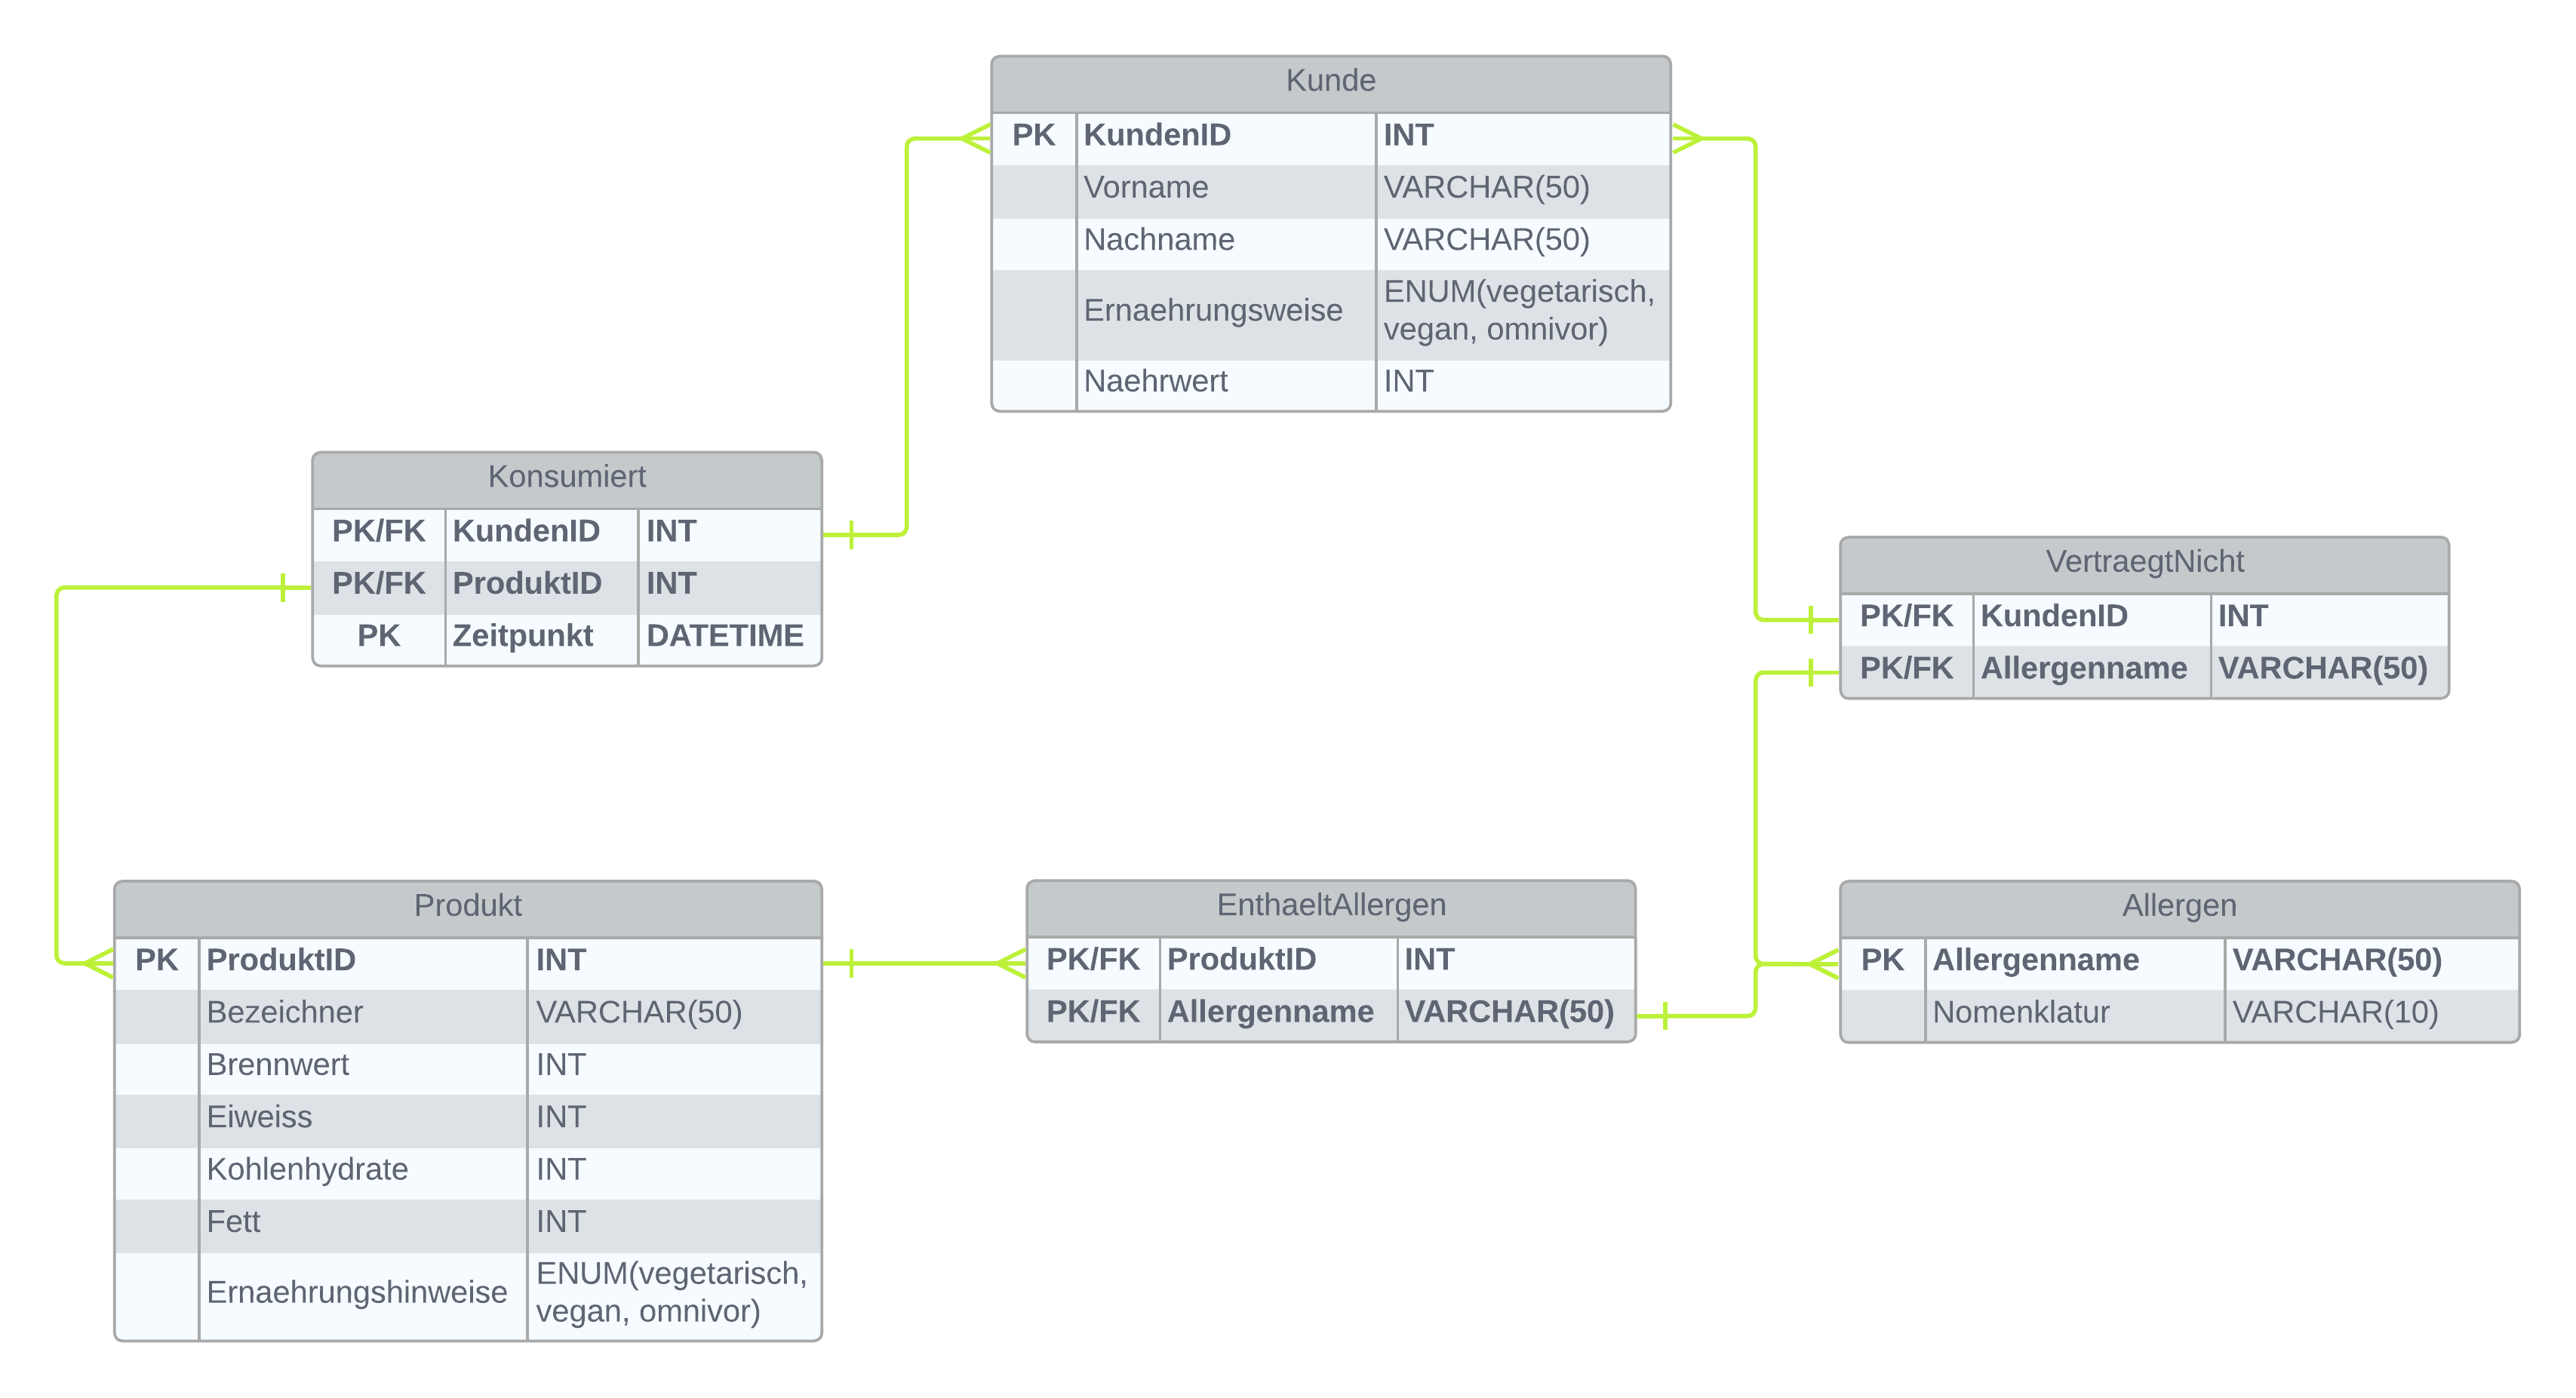
\includegraphics[width=0.9\textwidth]{images/neo4j_example_relational_model.png}
\end{figure}

\autoref{fig:relationalModelNeo4j} shows the relational model of a food consumption database. It consists of three main tables, \textit{Kunde}, \textit{Produkt}, and \textit{Allergen} that are connected by the link tables \textit{Konsumiert}, \textit{VertraegtNicht}, and \textit{EnthaeltAllergen}. The link tables are used to map the many-to-many relationships between the main tables.

The \textit{Kunde} table contains customer data, such as first name, last name, or diet. The \textit{Produkt} table stores details about the products, such as name and nutritional values. Finally, in the \textit{Allergen} table, the name and nomenclature of the allergens are stored.

As a relationship between \textit{Kunde} and \textit{Produkt}, the table \textit{Konsumiert} stores which products a customer has consumed. It also has an additional column \textit{Zetipunkt} for the consumption date. The table \textit{VertraegtNicht} contains information about the allergens that customers are allergic to. Last, the table \textit{EnthaeltAllergen} stores the allergens that are contained in products.

\subsubsection*{Graph Model}

\begin{figure}[H]
    \centering
    \caption{Graph Model of the Food Consumption Database}\label{fig:graphModelNeo4j}
    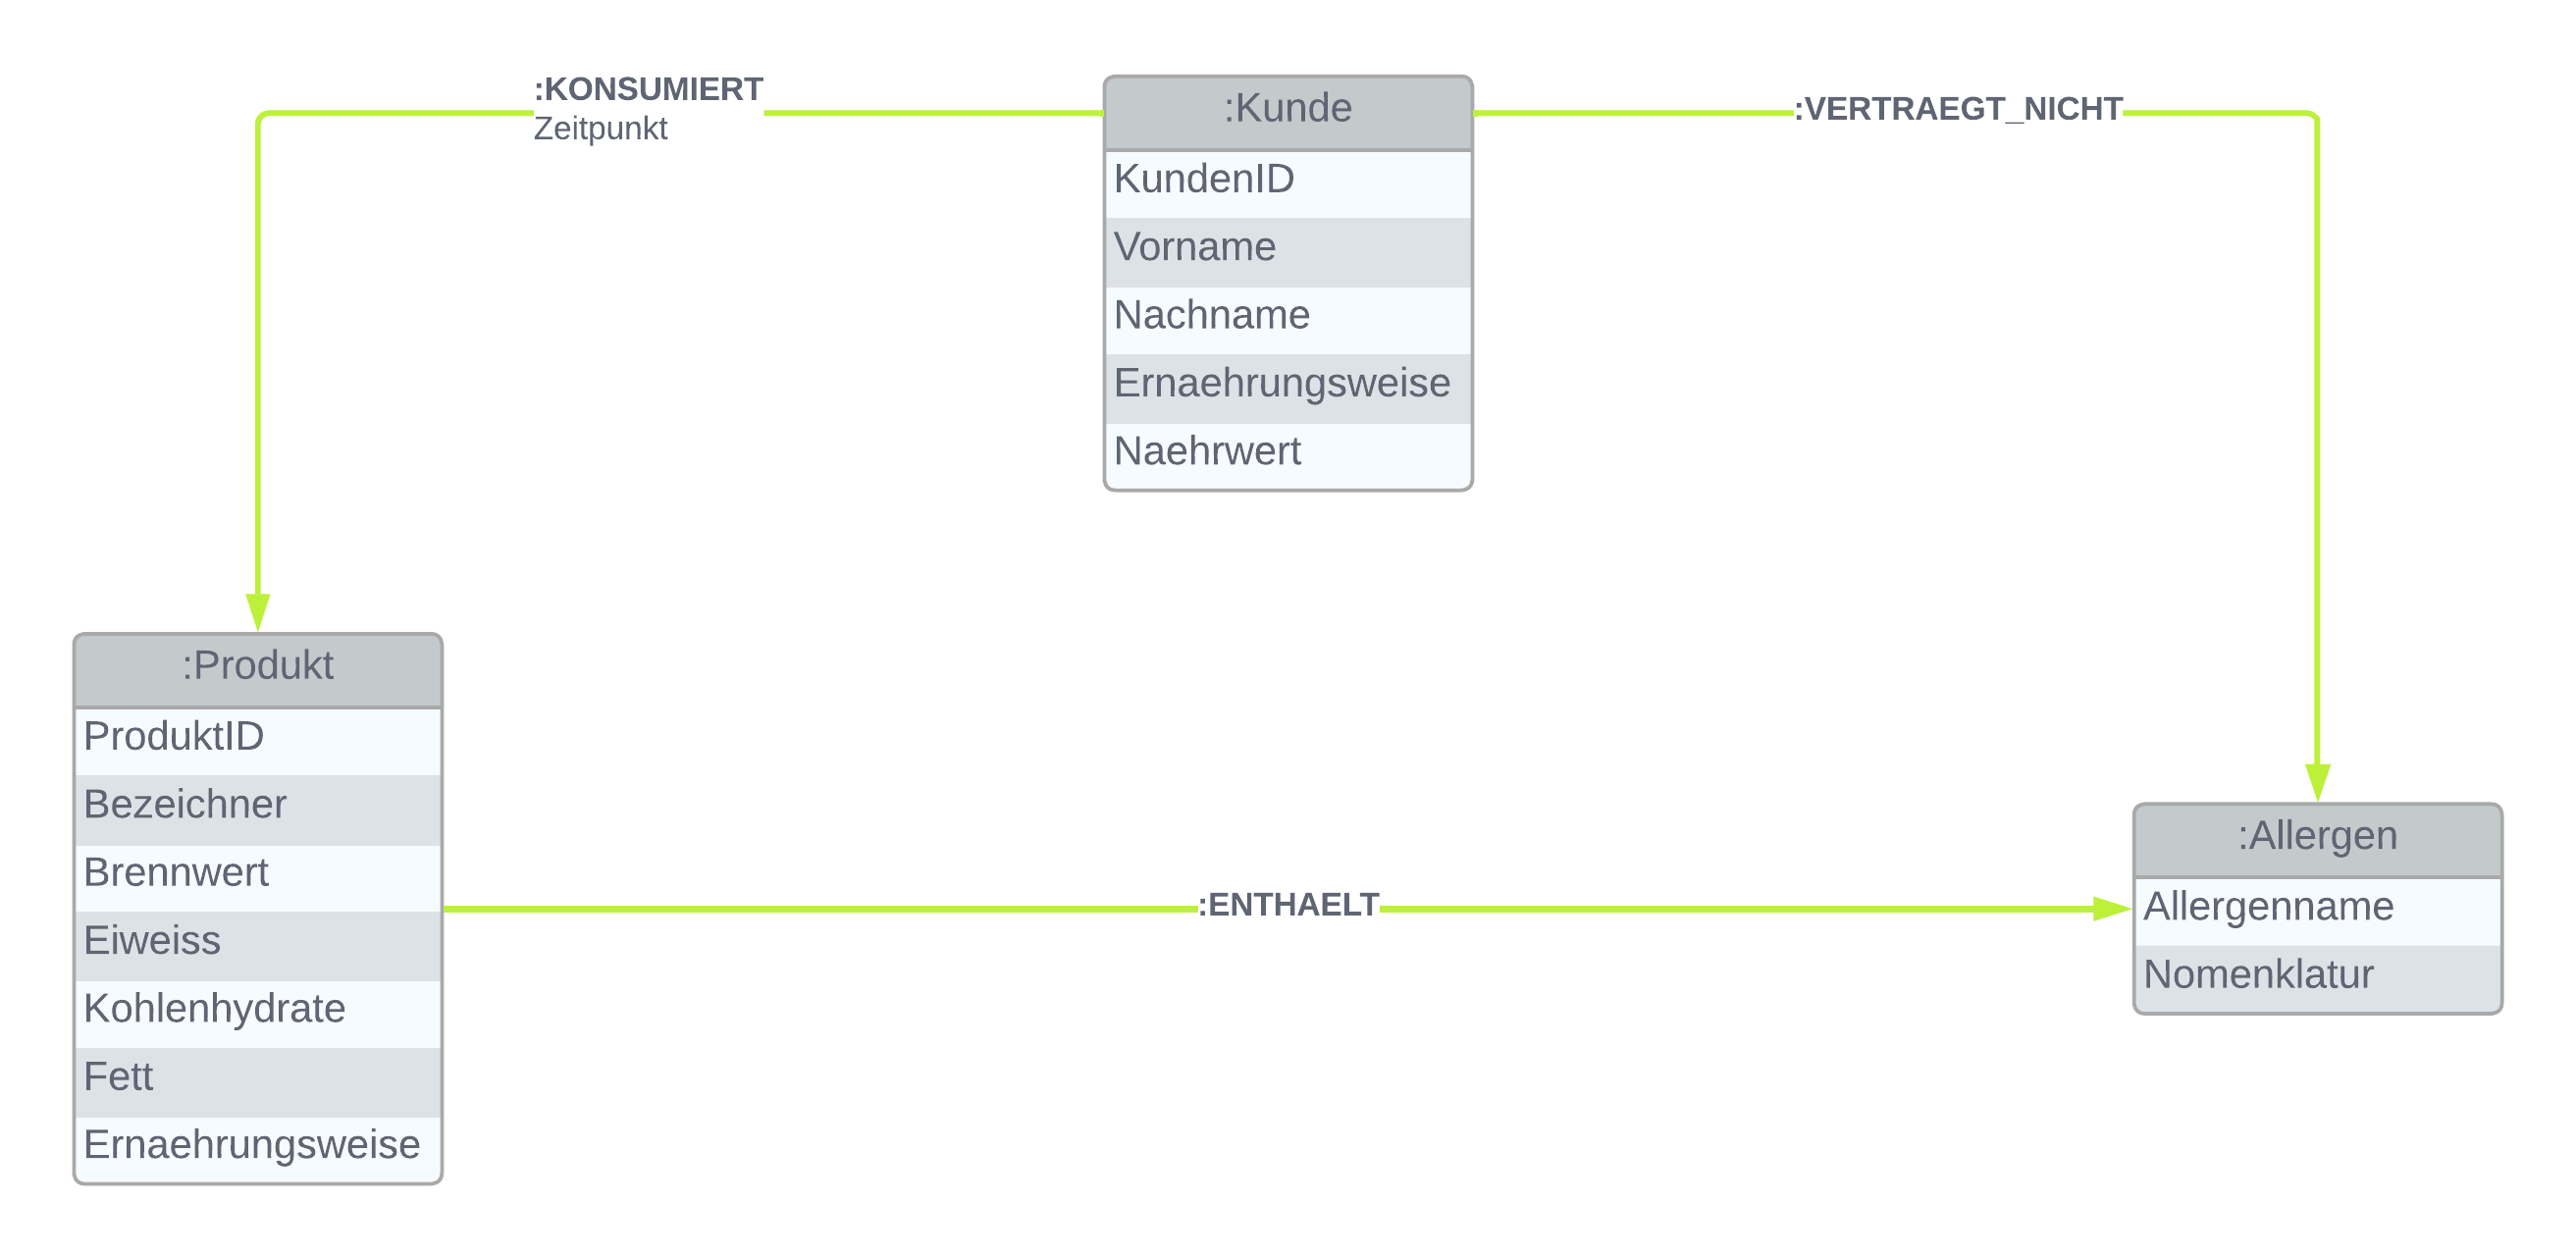
\includegraphics[width=0.9\textwidth]{images/neo4j_example_graph_model.png}
\end{figure}

\autoref{fig:graphModelNeo4j} illustrates a graph model based on the previously described relational food consumption database. The main tables \textit{Kunde}, \textit{Produkt}, and \textit{allergen} are now represented by a specific type of node with the table name as the label. It is essential to notice that in contrast to the relational model, where all data is stored in a single table, every row of a table is represented by a distinct node in the graph model. Since nodes in Neo4j can have properties, the column values of the original table can be stored as properties of the nodes.

In addition, the link tables \textit{Konsumiert}, \textit{VertraegtNicht}, and \textit{EnthaeltAllergen} are now represented by direct connections, so edges between nodes of the entities of a relationship. For example, the relationship between \textit{Kunde} and \textit{Produkt} is now represented by an edge between the nodes of the \textit{Kunde} and \textit{Produkt} labels. The edges are labeled with the name of the relationship, in this case \textit{Konsumiert}. This edge also has a property \textit{Zetipunkt} that stores the consumption date.

\subsubsection*{Key Takeaways}

When migrating from a relational database model to a graph database model, there are several essential steps to follow, as could be noted in the previous example. These include --- most important --- the use of node labels, the mapping of table entries to nodes, the usage of relationships instead of foreign keys, and the replacement of link tables with relationships \parencite{neo4j_docs_migration}.

In a graph database model, tables from the relational model are mapped to node labels. Each node label represents an entity type that can be used to query and analyze the data. In the example of the food consumption database, the \textit{Kunde} table would be mapped to a \textit{Kunde} node label, the \textit{Produkt} table to a \textit{Produkt} node label, and the \textit{allergen} table to an \textit{Allergen} node label.

In addition, for each row in a table, a separate node has to be created. The node is labeled with the name of the table, and the columns of the table are represented as properties of the node. In the previously shown example, a \textit{Kunde} node has properties such as \textit{Vorname}, \textit{Nachname}, or \textit{Ernaehrungsweise}, which were columns in the original relational schema.

In relational databases, one-to-one or one-to-many relationships can be expressed by adding a foreign key of one of the participating relationship tables to the other. However, in a graph database model, relationships can be expressed by direct connections through edges between nodes. Hence, foreign keys are not necessary anymore. Like nodes, relationships also have a label to distinguish different kinds. For example, a \textit{Konsumiert} relationship might connect a \textit{Kunde} node with a \textit{Produkt} node, representing the fact that the customer has consumed the product. This approach of realizing relationships enables more complex and flexible queries without joining tables.

Finally, for a many-to-many relationship in relational databases, there has to be a separate link table storing only foreign keys and potentially additional attributes of the relationship. In graph databases, these link tables can also be replaced with relationships. Since relationships can have properties, any attributes of the original link table can be stored this way. In that regard, Neo4j simplifies the data model and eliminates the need for additional join operations required in relational models. In the food consumption database example, the link table \textit{Konsumiert} can be replaced by an edge between the nodes \textit{Kunde} and \textit{Produkt} with the additional property \textit{Zeitpunkt}.

\subsection{Installation} \label{subsec:installationNeo4j}

Neo4j can be installed on a local machine for personal use either via the Desktop Application (e.g., \texttt{.exe}, AppImage) or the Linux package \parencite{neo4j_neo4j_nodate}. Neo4j can be deployed for production environments using Docker \parencite{neo4j_docs_introduction_nodate} or Kubernetes to scale the database horizontally.

As Neo4j is implemented in Java, a \ac{JDK} must be installed, although the containerized versions may already include one.

In this paper, we will deploy a single instance of Neo4j using a Docker container. The container exposes two ports: \num{7687} for the \ac{UI} to run Cypher queries and \num{7474} for the \ac{Bolt} used to communicate with the database.

\subsection{Cypher Examples} \label{subsec:queryingNeo4j}

We will use the graph model from \autoref{subsec:migrationRelationModelNeo4j} to create and query nodes.

\begin{code}[H]
    \caption{Cypher Query to create a node} \label{code:cypherCreateNode}
    \begin{minted}[linenos, breaklines]{cypher}
// Create :Kunde nodes
CREATE (FelixHoffmann:Kunde {KundenID: "42", Vorname: "Felix", Nachname: "Hoffmann", Ernaehrungsweise: "vegan", Naehrwert: 1337})

// Create :Produkt nodes
CREATE (BigMac:Produkt {ProduktID: "1", Name: "Big Mac", Naehrwert: 257})

// Create :Allergen nodes
CREATE (GlutenhaltigesGetreide:Allergen {Allergenname: "Glutenhaltiges Getreide", Nomenklatur: "gluten"})

// Create :Konsumiert relationship
CREATE (FelixHoffmann)-[:Konsumiert {datum: "2019-01-01"}]->(BigMac)
    \end{minted}
\end{code}

\autoref{code:cypherCreateNode} shows a simple Cypher query to create multiple nodes and a relationship. The \texttt{CREATE} keyword starts the query, followed by a unique key for the node and the node type specified by the \texttt{:} symbol and its label. We can then specify attributes related to the node, such as \texttt{Vorname} set to \texttt{Felix} and \texttt{Nachname} set to \texttt{Hoffmann}. Lastly, the \texttt{CREATE} keyword and the relationship between two nodes are defined using an arrow syntax. The relationship label is set to \texttt{Konsumiert}, and the \texttt{datum} attribute is set to \texttt{2019-01-01}.

We then created additional nodes and relationships, resulting in the following graph. To retrieve this graph, we run the query \texttt{MATCH (n) RETURN n}, which matches all nodes in the database and returns them.

\begin{figure}[H]
    \centering
    \caption{Graph including all nodes in the database} \label{fig:neo4jGraph_1}
    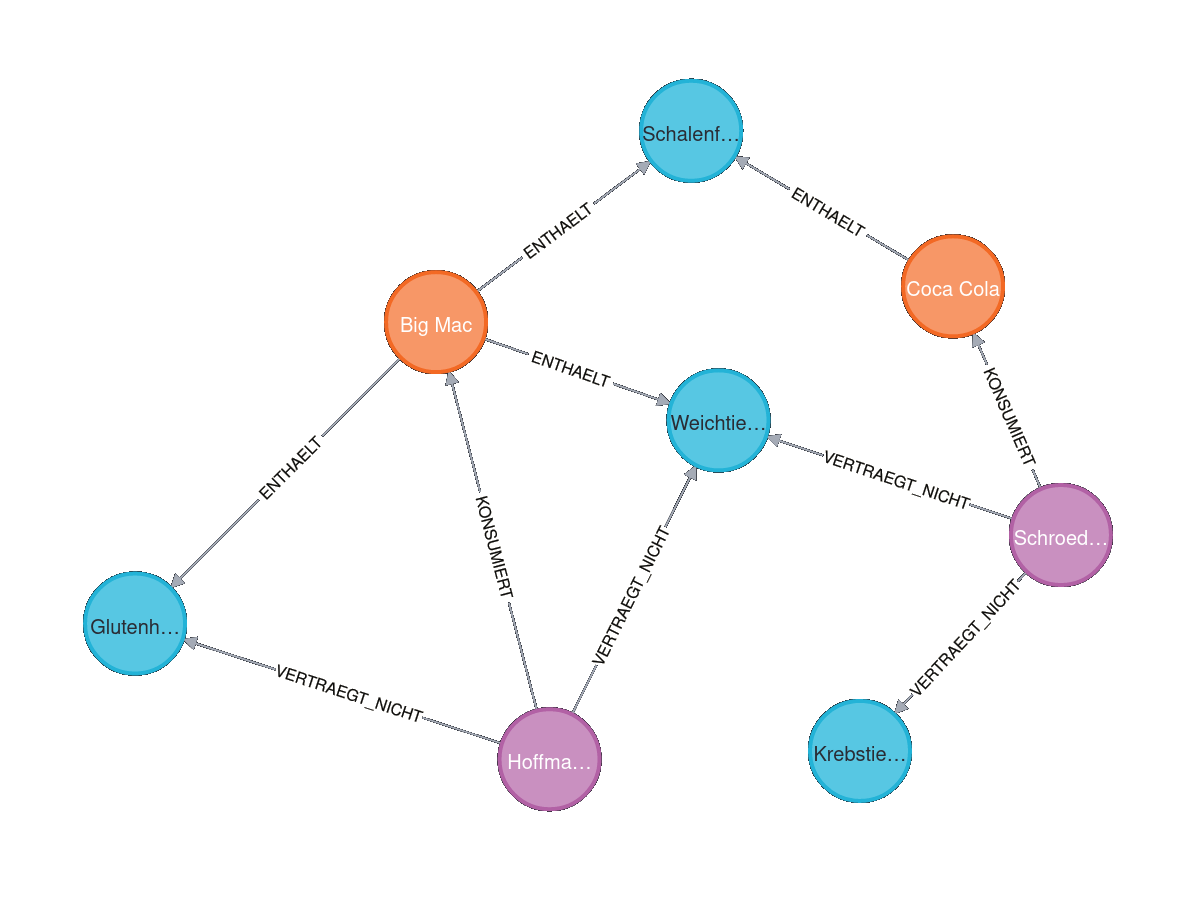
\includegraphics[width=0.7\textwidth]{images/neo4j_example_graph_1.png}
\end{figure}

For this example, we created additional nodes and relationships. The query result is shown in \autoref{fig:neo4jGraph_1}. The graph shows all nodes and relationships in the database. This graph can be retrieved by running \texttt{MATCH (n) RETURN n}. The \texttt{MATCH} keyword is used to specify the pattern of the query. In this case, we want to match all nodes in the database. The \texttt{RETURN} keyword is used to specify the result of the query. In this case, we want to return all nodes in the database.

\begin{code}[H]
    \caption{Cypher Query to select allergic reactions} \label{code:cypherFindAllergicReactions}
    \begin{minted}[linenos, breaklines]{cypher}
// Detect customer who ate a product that contains an allergen that he is not able to eat
MATCH (k:Kunde)-[:Konsumiert]->(p:Produkt)
(k)-[:VERTREAGT_NICHT]->(a:Allergen)<-[:ENTHAELT]-(p)
RETURN k, a, p
    \end{minted}
\end{code}

Next, we run a query to find all allergic reactions, shown in \autoref{code:cypherFindAllergicReactions}. The \texttt{MATCH} keyword specifies the query's pattern to match all nodes of types \texttt{Kunde} and \texttt{Produkt} connected by a relationship of type \texttt{Konsumiert}. We then specify that the customer does not tolerate an allergen and that the product contains this allergen. Lastly, we want to return the customer and the product.

\begin{figure}[H]
    \centering
    \caption{Graph of a selection of Nodes} \label{fig:neo4jGraph_2}
    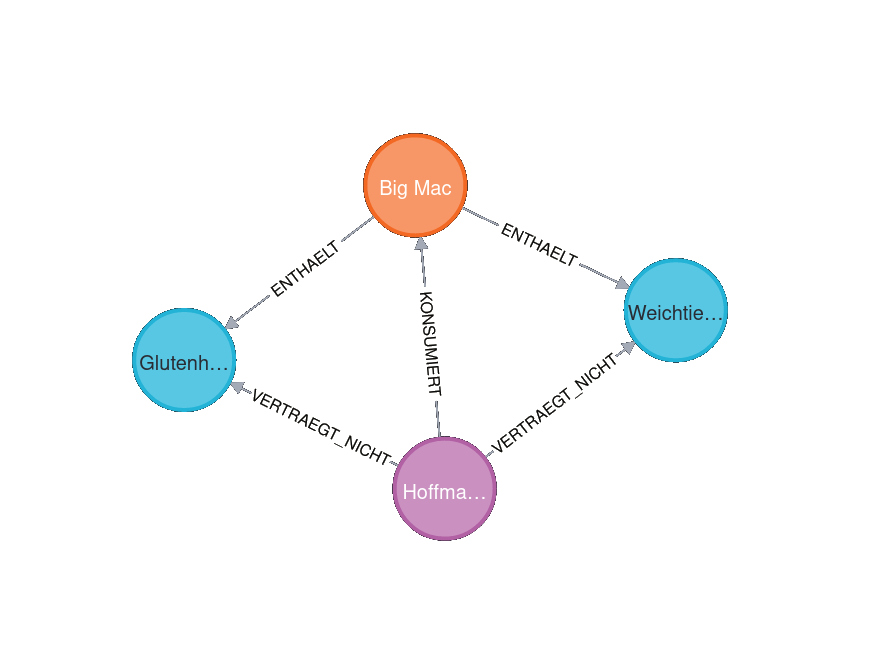
\includegraphics[width=0.6\textwidth]{images/neo4j_example_graph_2.png}
\end{figure}

\section{Reflection} \label{sec:reflectionNeo4j}

In this section, we have discussed Neo4j, a graph database management system designed to handle highly interconnected data efficiently. We have explored the features and capabilities of Neo4j, including its query language, data modeling, and data analysis tools. We have also examined its performance and scalability, as well as its consistency and availability trade-offs. Overall, Neo4j is a powerful tool that can be used in various domains, including social networks, recommendation systems, and fraud detection. However, it may only be suitable for some types of data, and its adoption may depend on the specific requirements of each use case.

\subsection{CAP Theorem} \label{subsec:capTheoremNeo4j}

Neo4j is normally classified as a \ac{CA}-database, which means that it offers consistency and availability at the expense of partition tolerance. This is usually justified by Neo4j not offering sharding \parencite{cap_neo4j}. While this is true for the community edition, it does not apply to the enterprise edition, which introduced sharding about two years ago. Therefore, Neo4j is usually used as a \ac{CA}-database, but in rare cases, it might also be used as a \ac{CP} or \ac{AP} database \parencite{consistency_models_cap_neo4j}.

\subsection{Conclusion} \label{subsec:conclusionNeo4j}

In conclusion, Neo4j is a powerful graph database system based on graph theory, which makes it particularly suited for managing and analyzing highly connected data. Its optimized query language, Cypher, enables efficient data retrieval from the database. However, it should be noted that graph databases may not be optimal for analyzing all nodes in one query, and relational models can be easily converted to graph models using Neo4j. Overall, Neo4j's innovative design and features make it an ideal choice for applications that require efficient management and analysis of complex relationships and data structures.

% Neo4j is a graph database which means that it is based on the graph theorem. It supports the query language Cypher, which is optimized for querying graph databases. When dealing with highly connected data, graph databases such as Neo4j are often a good fit because the data structure of these databases is optimized for it. Further, the most common queries should only analyze parts of the graph because graph databases are slower than relational databases if all nodes are accessed in one query. Lastly, converting a relational model into a graph model is possible. 
